% Chapter 1

\chapter{Dispersive Materials} % Write in your own chapter title
\label{Chapter4}
\lhead{Chapter 3. \emph{Dispersive Materials}} % Write in your own chapter title to set the page header

In general light travels as a polychromatic waves - containing several different frequencies. In general each frequency travels at a different speed in a medium. The material parameters depend on the frequency of the radiation.

\section{The Drude Model}

The drude model was initially proposed in *** based on the kinetic theory of gases [citation]. In the drude model a metal is modelled as a fixed lattice of positively charged ions in a sea of negatively charged valance or conduction (in a metal) electrons which are free to move.

%TODO  - direct quote - IntriaPaper DGTD dispersive
Assumptions:
• The electrons description is non-relativistic;
• The only considered interactions are the electron/wave and the electron/ion ones;
• The electron/ion collisions are instantaneous and random events, and their probability of happening during a dt amount of time is equal to dt 1;
τf
• After an electron/ion collision, the new velocity and direction of the electron are inde-
pendant of those before the collision.


Under these hypotheses, the frequency dependence of the medium permittivity can be de- duced from the equations of motion.
%TODO - end direct quote

When subjected to a constant external electric field $\mathbf{E}$ the displacement of the heavy valence ions from their equilibtrium position is assume to be negligable whilst the electrons move significantly from their equilibrium position in response to an externally applied field. This results in an additional electric field $\mathbf{P}$ due to material response to the applied field $\mathbf{E}$ orientated in the opposite direction resulting in a total field given by the electric displacement field $\mathbf{D}$ where:

$$
\mathbf{D} = \epsilon_0 \mathbf{E} + \mathbf{P}
$$

Note that usually the signs of $\mathbf{P}$ and $\mathbf{E}$ will be opposite - resulting in an induced field that opposes the applied field and consequentially a reduced field in the medium.

% TODO: Is it accurate to describe the displacement electric field as the total electric field....?

For a constant or slow-varying field with respect to the material response time $\tau$ the polarisation of the material $\mathbf{P}$ will be proportional to the applied electric field and can be described as a constant of proportionality $\chi$, known as the electric susceptibility which describes how susceptible the material is to polarisation. $\mathbf{P}$ can be written as:

$$
\mathbf{P} = \chi \mathbf{E}
$$

$\chi$ is not always constant - and in general is a tensor.

Furthermore the movement of electrons from their zero-field equlibrium positions to the equilibrium positions under the applied field $\mathbf{E}$ could take some finite time $\tau$ (characteristic time). For an applied electric field $\mathbf{E}$ which is changing sufficiently quickly this time needs to be accounted for and $\chi$ may not be described as simply by a constant since it clearly depends on the history of the mediums polarisation.

TODO - derivation from equations of motion to conservation form....find a nice way of doing this....

\section{Beyond the Drude Model}
- what about the Lorentz model
- Drude/Lorentz model
- Debye model
- Generalised dispersion

\section{Non-Dimensionalization of Drude Model}
We define the following dimensionless units for a system with a characteristic length L:
$$
t' = \frac{ct}{L}
$$

$$
\mathbf{x'} = \frac{\mathbf{x}}{L}
$$

$$
\mathbf{E'} = \mathbf{E}\sqrt{\frac{\epsilon_0}{\mu_0}}
$$

$$
\mathbf{J'} = L\mathbf{J}
$$

\section{Results}

\begin{figure}
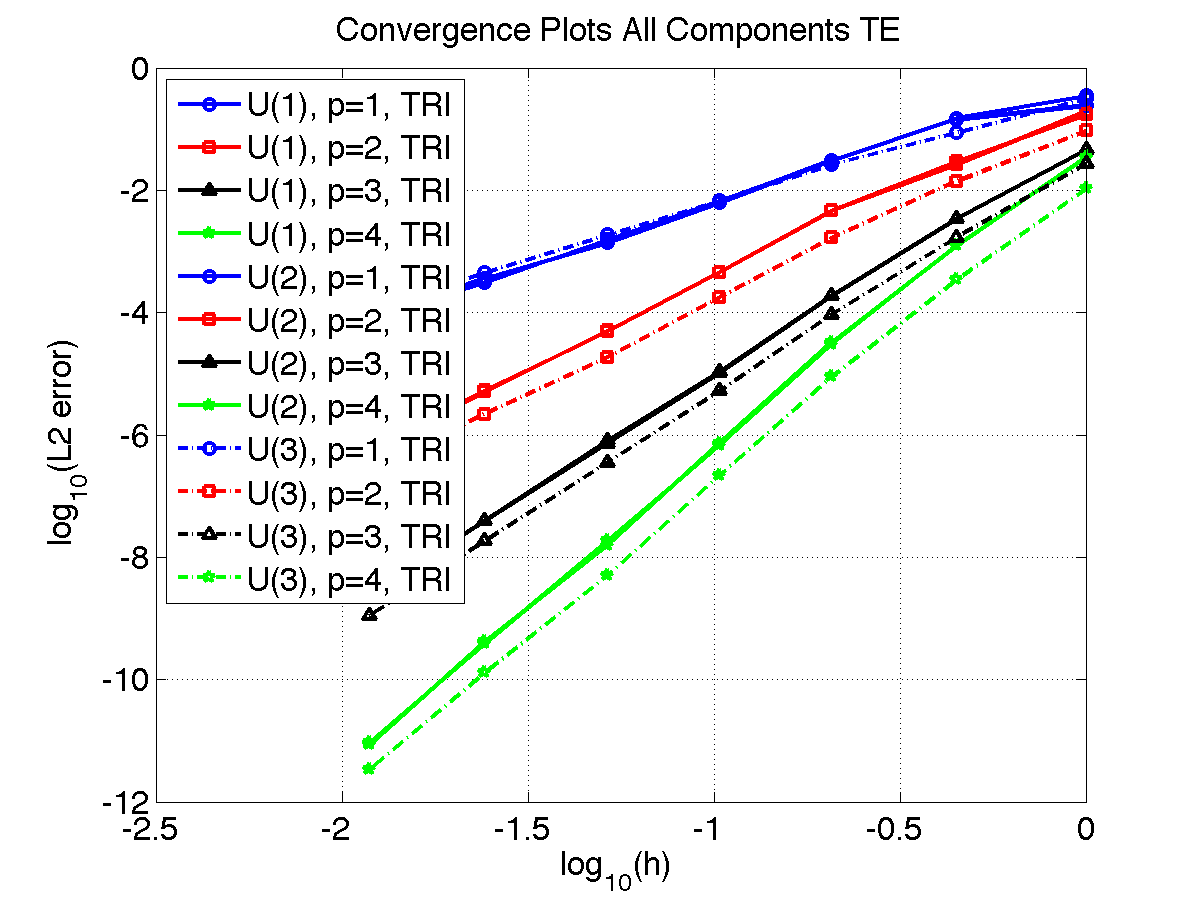
\includegraphics[width=\textwidth]{Figures/2D_DispersivePlate/convergenceStudies/convergenceAllComponents/L2vsH_TE.png}
\caption{Convergence plots fo TE validation case}
\end{figure}

\begin{figure}
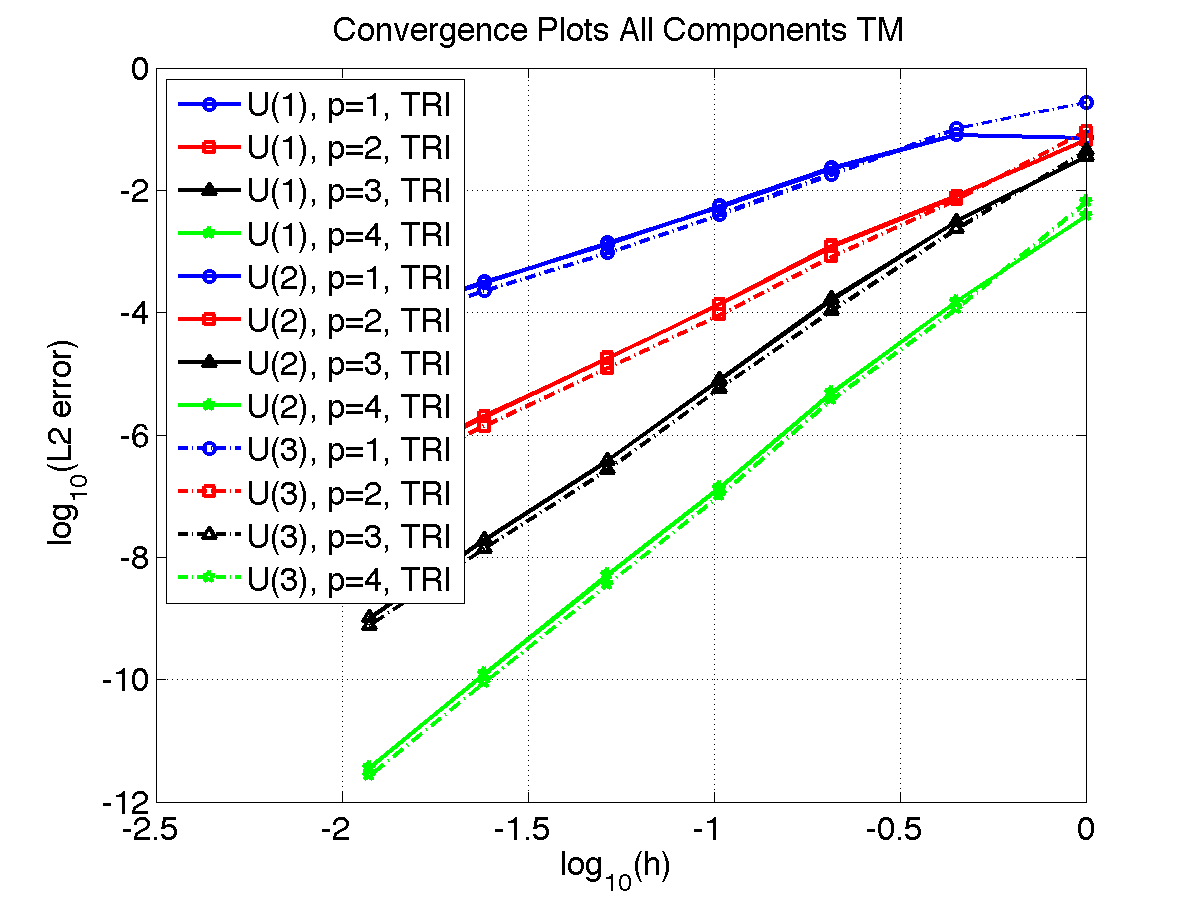
\includegraphics[width=\textwidth]{Figures/2D_DispersivePlate/convergenceStudies/convergenceAllComponents/L2vsH_TM.png}
\caption{Convergence plots fo TM validation case}
\end{figure}

\begin{figure}
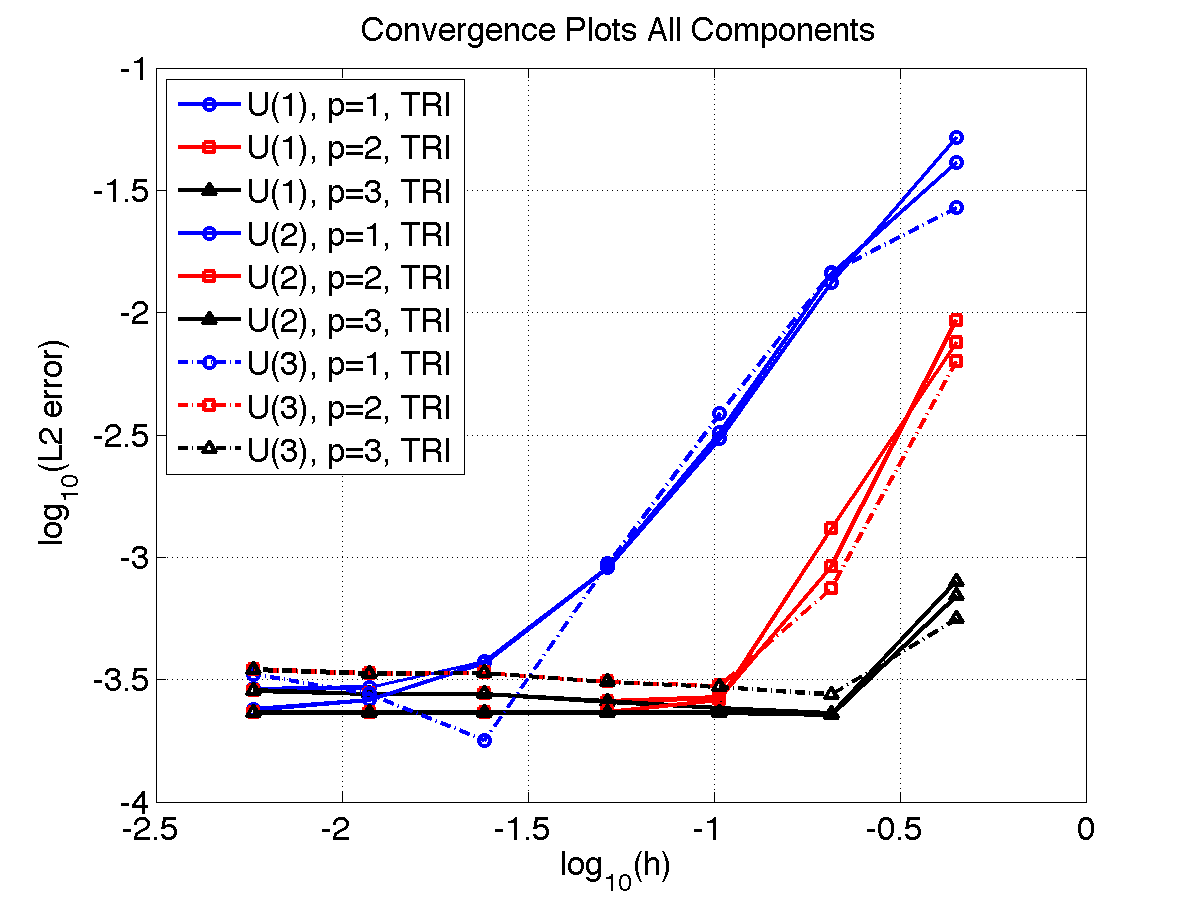
\includegraphics[width=\textwidth]{Figures/2D_DispersivePlate/convergenceStudies/convergenceAllComponents/L2vsH.png}
\caption{Convergence plots for all component case}
\end{figure}

\clearpage
\section{Error Plots}

\begin{figure}
\includegraphics[width=\textwidth]{Figures/2D_DispersivePlate/convergenceStudies/ErrorPlots/convergencePlots_dat_dispersiveSquareQUA_H3_p3_TE_iComp1.png}
\end{figure}

\begin{figure}
\includegraphics[width=\textwidth]{Figures/2D_DispersivePlate/convergenceStudies/ErrorPlots/convergencePlots_dat_dispersiveSquareQUA_H3_p3_TE_iComp2.png}
\end{figure}

\begin{figure}
\includegraphics[width=\textwidth]{Figures/2D_DispersivePlate/convergenceStudies/ErrorPlots/convergencePlots_dat_dispersiveSquareQUA_H3_p3_TE_iComp3.png}
\end{figure}

\begin{figure}
\includegraphics[width=\textwidth]{Figures/2D_DispersivePlate/convergenceStudies/ErrorPlots/convergencePlots_dat_dispersiveSquareQUA_H3_p4_TE_iComp1.png}
\end{figure}

\begin{figure}
\includegraphics[width=\textwidth]{Figures/2D_DispersivePlate/convergenceStudies/ErrorPlots/convergencePlots_dat_dispersiveSquareQUA_H3_p4_TE_iComp2.png}
\end{figure}

\begin{figure}
\includegraphics[width=\textwidth]{Figures/2D_DispersivePlate/convergenceStudies/ErrorPlots/convergencePlots_dat_dispersiveSquareQUA_H3_p4_TE_iComp3.png}
\end{figure}

\begin{figure}
\includegraphics[width=\textwidth]{Figures/2D_DispersivePlate/convergenceStudies/ErrorPlots/convergencePlots_dat_dispersiveSquareQUA_H3_p4_TM_iComp1.png}
\end{figure}

\begin{figure}
\includegraphics[width=\textwidth]{Figures/2D_DispersivePlate/convergenceStudies/ErrorPlots/convergencePlots_dat_dispersiveSquareQUA_H3_p4_TM_iComp2.png}
\end{figure}

\begin{figure}
\includegraphics[width=\textwidth]{Figures/2D_DispersivePlate/convergenceStudies/ErrorPlots/convergencePlots_dat_dispersiveSquareQUA_H3_p4_TM_iComp3.png}
\end{figure}

\begin{figure}
\includegraphics[width=\textwidth]{Figures/2D_DispersivePlate/convergenceStudies/ErrorPlots/convergencePlotsTRI_TM_dat_dispersiveSquareTRI_H5_p3_TM_iComp1.png}
\end{figure}

\begin{figure}
\includegraphics[width=\textwidth]{Figures/2D_DispersivePlate/convergenceStudies/ErrorPlots/convergencePlotsTRI_TM_dat_dispersiveSquareTRI_H5_p3_TM_iComp2.png}
\end{figure}

\begin{figure}
\includegraphics[width=\textwidth]{Figures/2D_DispersivePlate/convergenceStudies/ErrorPlots/convergencePlotsTRI_TM_dat_dispersiveSquareTRI_H5_p3_TM_iComp3.png}
\end{figure}

\begin{figure}
\includegraphics[width=\textwidth]{Figures/2D_DispersivePlate/convergenceStudies/ErrorPlots/dispersiveSquareQUA_H1_p3_TE_iComp1.png}
\end{figure}

\begin{figure}
\includegraphics[width=\textwidth]{Figures/2D_DispersivePlate/convergenceStudies/ErrorPlots/dispersiveSquareQUA_H1_p3_TE_iComp2.png}
\end{figure}

\begin{figure}
\includegraphics[width=\textwidth]{Figures/2D_DispersivePlate/convergenceStudies/ErrorPlots/dispersiveSquareQUA_H1_p3_TE_iComp3.png}
\end{figure}

\clearpage

\begin{figure}
\includegraphics[width=\textwidth]{Figures/2D_DispersivePlate/convergenceStudies/ErrorPlots/dispersiveSquareQUA_H3_p1_TE_iComp1.png}
\end{figure}

\begin{figure}
\includegraphics[width=\textwidth]{Figures/2D_DispersivePlate/convergenceStudies/ErrorPlots/dispersiveSquareQUA_H3_p1_TE_iComp2.png}
\end{figure}

\begin{figure}
\includegraphics[width=\textwidth]{Figures/2D_DispersivePlate/convergenceStudies/ErrorPlots/dispersiveSquareQUA_H3_p1_TE_iComp3.png}
\end{figure}

\begin{figure}
\includegraphics[width=\textwidth]{Figures/2D_DispersivePlate/convergenceStudies/ErrorPlots/dispersiveSquareQUA_H3_p3_TE_iComp1.png}
\end{figure}

\begin{figure}
\includegraphics[width=\textwidth]{Figures/2D_DispersivePlate/convergenceStudies/ErrorPlots/dispersiveSquareQUA_H3_p3_TE_iComp2.png}
\end{figure}

\begin{figure}
\includegraphics[width=\textwidth]{Figures/2D_DispersivePlate/convergenceStudies/ErrorPlots/dispersiveSquareQUA_H3_p3_TE_iComp3.png}
\end{figure}

\begin{figure}
\includegraphics[width=\textwidth]{Figures/2D_DispersivePlate/convergenceStudies/ErrorPlots/dispersiveSquareQUA_H3_p3_TM_iComp1.png}
\end{figure}

\begin{figure}
\includegraphics[width=\textwidth]{Figures/2D_DispersivePlate/convergenceStudies/ErrorPlots/dispersiveSquareQUA_H3_p3_TM_iComp2.png}
\end{figure}

\begin{figure}
\includegraphics[width=\textwidth]{Figures/2D_DispersivePlate/convergenceStudies/ErrorPlots/dispersiveSquareQUA_H3_p3_TM_iComp3.png}
\end{figure}

\begin{figure}
\includegraphics[width=\textwidth]{Figures/2D_DispersivePlate/convergenceStudies/ErrorPlots/dispersiveSquareTRI_H5_p3_TE_iComp1.png}
\end{figure}

\begin{figure}
\includegraphics[width=\textwidth]{Figures/2D_DispersivePlate/convergenceStudies/ErrorPlots/dispersiveSquareTRI_H5_p3_TE_iComp2.png}
\end{figure}

\begin{figure}
\includegraphics[width=\textwidth]{Figures/2D_DispersivePlate/convergenceStudies/ErrorPlots/dispersiveSquareTRI_H5_p3_TE_iComp3.png}
\end{figure}

\begin{figure}
\includegraphics[width=\textwidth]{Figures/2D_DispersivePlate/convergenceStudies/ErrorPlots/moreSnapshotsForErrorMovie_dat_dispersiveSquareQUA_H3_p3_TM_iComp1.png}
\end{figure}

\begin{figure}
\includegraphics[width=\textwidth]{Figures/2D_DispersivePlate/convergenceStudies/ErrorPlots/moreSnapshotsForErrorMovie_dat_dispersiveSquareQUA_H3_p3_TM_iComp2.png}
\end{figure}

\begin{figure}
\includegraphics[width=\textwidth]{Figures/2D_DispersivePlate/convergenceStudies/ErrorPlots/moreSnapshotsForErrorMovie_dat_dispersiveSquareQUA_H3_p3_TM_iComp3.png}
\end{figure}